%\right) %\documentclass[conference]{IEEEtran}
%\documentclass[10pt, conference, letterpaper]{IEEEtran}
\documentclass[conference]{IEEEtran}


\usepackage{amsfonts}
\usepackage{amssymb}
\usepackage{amsmath}
\usepackage{algorithm}
\usepackage[noend]{algorithmic}
\usepackage{color}
\usepackage{graphicx}
\usepackage{subfigure}
\usepackage{comment}
\usepackage[strings]{underscore}
\usepackage{comment}
\usepackage{url}



\hyphenation{op-tical net-works semi-conduc-tor}
\setlength{\parskip}{0.1em}
\renewcommand{\baselinestretch}{1}

\begin{document}


\title{DSP Matlab Assignment \\Designing Low Pass Filters with MATLAB}
\author{\IEEEauthorblockN{Vincent Martin}
\IEEEauthorblockA{
Department of Electrical Engineering\\
Temple University, Philadelphia, PA, USA \\
Email: \{vince.p.martin\}@temple.edu }
}

\maketitle

%\vspace*{-0.5cm}
\begin{abstract}


\end{abstract}
This report reviews how MATLAB can be used to construct a low pass filter. The construction of such a filter is used on a noisy .wav audio file to determine what its contents are. MATLAB code is included.

\section{Introduction}
Filters are used to alter data that are passed through it based on the frequency of that data. For example, a low pass filter would be used to pass only values that are determined to be under the set cutoff frequency that the designer has determined. Additionally there are other filters such as high pass filters that pass only data that is above the cutoff frequency and finally, band pass filters that are a combination of both low and high pass filters. This report will walk through the construction of a low pass filter by using one to filter a noisy .wav file.

\section{Construction of the Low Pass Filter}
Constructing the low pass filter in MATLAB requires that we determine values for the pass band frequency (Fpass), stop band frequency (Fstop), pass band ripple (Apass) and the stop band attenuation (Astop). Figure displays all of these values visually.

%\begin{figure}[H]
%\centering
%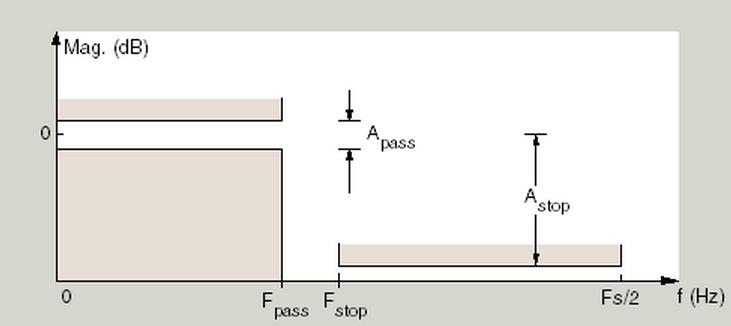
\includegraphics[width=3.0in]{./figures/filter.png}
%\caption{Mixed mode processing.}
%\label{figure:filter}
%\end{figure}


\subsection{Determining the Frequency Stop



\section{Conclusion}

{\footnotesize
\bibliographystyle{IEEEtran}
\bibliography{glass-video}
}
\end{document}


